\section{Tackling the Challenges: The Design of SemNotes}
\label{sec:semnotesdesign}

We use our note-taking application, SemNotes, to describe the general principles we used for designing an application for the Semantic Desktop. Note-taking is a good general use case for the Semantic Desktop because the information contained in notes is not restricted to a specific domain. Personal notes are naturally connected to the user's context, and can thus be meaningfully interconnected with much of the existing network of personal data on the desktop.

We divided the design into specialised modules. Each module handles a set of related tasks. We describe the modules as they would be for a general semantic application, followed by a more specific description about the implementation of SemNotes in the next section.
 
\subsection{Data Representation} 

This module handles the vocabulary of the application: the \emph{data types} around which the application is centred, and the kind of \emph{metadata} that is needed for them. To enable other Semantic Desktop applications to understand the data produced, as well as for our application to understand data from the underlying Semantic Desktop, the best practice is to reuse existing desktop ontologies where possible. The basic data type handled by SemNotes is the note, represented by a short snippet of text containing personal information. 

\subsection{Data Management} 

This module manages the life-cycle of the semantic data that the application handles, by enabling the transition between the phases of the life-cycle. We adapted the Abstract Data Life-Cycle Model \cite{MoellerPhDThesis2009} to illustrate a comprehensive workflow for Semantic Desktop data, from its creation to its termination. Figure~\ref{fig:datalifecycle} shows the phases and transitions between them, focusing on the possible actions that the user can execute, and hence, that a semantic application could support.

\begin{figure}[htb]
 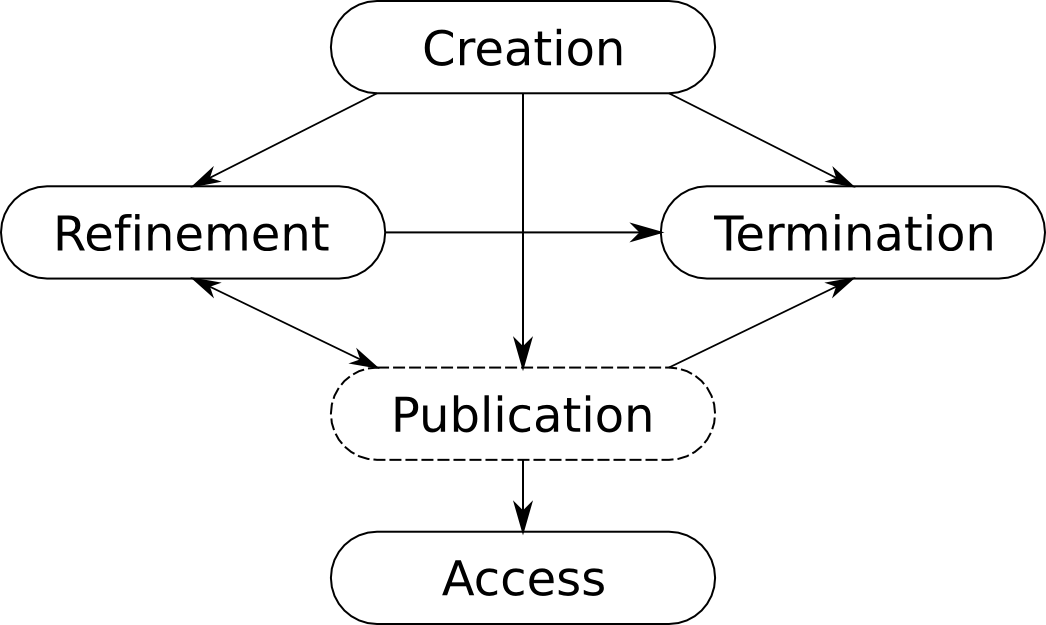
\includegraphics[width=0.7\linewidth]{chapters/core/img/lifecycle}
\caption{Semantic Desktop data life-cycle.}
\label{fig:datalifecycle}
\end{figure} 

\begin{description}
 \item[Creation.] Most often creation implies creating a new resource, of a given type. However, the import of existing data from other applications or formats (e.g. crawlers) is also included here.
 \item[Refinement.] This phase includes any activities that make changes to existing data. It also contains the creation and deletion of links between existing resources, although alternatively they can be included in the Creation or Termination phases, as links are data too. 
 \item[Access.] This phase is represented by accessing the data through either querying or browsing. Because we are discussing interlinked data, accessing a piece of semantic data implies recursively accessing the sub-graph of resources semantically related to it. How much of the sub-graph is traversed can vary, and further traversal by the user should be supported and encouraged. 
 \item[Termination.] In this phase the data is deleted from the system. As with the access phase, rules must be defined to determine how much of the dataset a deletion will affect---e.g. it might make sense to delete all the subtasks of a task when the parent is deleted, but not to delete the documents related to the task.
 \item[Publication.] This phase represents making the data accessible to users from outside the system. Also included here is exporting the data to other formats and applications. When handling semantic personal data, applications should ensure that sensitive data is well protected against unauthorised or accidental publication. 
\end{description}

Furthermore, this module handles where and how the data is stored. The Semantic Desktop provides the framework for storing semantic data, therefore it is best that the central desktop repository be used, when practical. This enables easier interlinking with the rest of the data. In the case of SemNotes, the notes and all the metadata about them are stored in the desktop repository. 

\subsection{Interlinking} 

The interlinking module is logically a sub-module of the Data management one, as it specifically manages a part of the refinement phase of the data life-cycle. However, because it is an important part of any semantic application, relating to the first two challenges listed in Section \ref{sub:appchallenges}, we describe it as a standalone module. The interlinking module effectively realises the goal of integrating the new semantic data into the pool of existing linked desktop data. The functionalities offered can vary from simple automatic linking of new resources to a specified context or to their author, to complex extraction and inference of new relations and resources.  This module provides the feature that sets SemNotes apart from other note-taking tools, the interlinking of the notes with the desktop resources mentioned in them. In our application, there are two sub-modules, that handle \begin{inparaenum}[(i)] \item entity recognition, and \item information extraction\end{inparaenum}, suggesting 
possible new connections to be created by the user.
 
\subsection{Visualisation} 

The visualisation module presents the data to the user in a simple, yet useful and versatile way. It addresses the third challenge listed above: designing the interface. Depending on the application, the visualisation can include \emph{aggregated} views on the data, and \emph{filters}. Faceted search \cite{Yee2003} has proven useful for semantic data, and it can be used to present the interlinked information to the user in a meaningful way. In SemNotes, the data that needs to be visualised is basically an enhanced version of a list of notes, with sorting and filtering. The module also provides the note editor. An important part of the module is displaying the recommendations for interlinking, a difficult task due to the heterogeneous nature of the information to be presented in a uniform, uncluttered way.

We describe how we tackled the last question --- the evaluation of the application --- in Section \ref{sec:semnotesevaluation}. 
